\section{Additional favorable results and supporting statistics}
\label{sec:app-experiments}

\subsection{Calibration and evaluation protocol}
\label{sec:app-protocol}

Coefficients are always fitted on unlabeled WikiText-103 \citep{merity2017pointer}, and
never on task data. Evaluation protocols differ by run, and we state them separately
rather than as one global constant.

\paragraph{0.5B layer analysis and \Cref{tab:selection}.} Coefficients are fitted on
16 WikiText-103 sequences of length 512; $P_\ell$ and the NLL-recovery
fractions are scored on 16 \emph{disjoint held-out WikiText-103} sequences. This is
a development protocol: it is the split on which layers are selected and the ridge is
chosen, and no number reported from it is a test-set number.

\paragraph{0.5B composition (\Cref{tab:main}).} Coefficients are fitted on the same
16 WikiText-103 sequences, but NLL is reported on the \emph{WikiText-2 test} split
(32 sequences), and downstream accuracy on 100 examples per task.

\paragraph{1.5B and \topscale.} Coefficients are fitted on 32 WikiText-103
sequences of length 1024; NLL is reported on the WikiText-2 test split and accuracy
on 300 examples per task.

Task evaluation uses fixed example IDs and seed 42 throughout. Statistics for
\cref{eq:fit} are accumulated in FP64, so no hidden states need to be stored. The 0.5B
runs use FP32 on an NVIDIA TITAN X (Pascal) GPU; 1.5B and \topscale use BF16 on a single
NVIDIA RTX 3090. No configuration uses FlashAttention, so we use the reference attention
implementation everywhere. Absolute latencies are specific to this hardware, though the
relative comparison between methods is not.

\subsection{Latency measurement}
\label{sec:app-latency}

We report \emph{prefill} latency only: a forward pass with
\texttt{use\_cache=False}, batch size 8, at sequence lengths 512 and 2048,
with 10 warm-up iterations followed by 30 measured iterations, and
\texttt{torch.cuda.synchronize()} around each timed region. We report the median
and interquartile range over synthetic inputs, on an NVIDIA RTX 3090 in BF16 with eager
attention, using the \Cref{tab:main} $k=4$ layer set, for both Qwen2.5-1.5B and
Qwen2.5-7B. On 7B at sequence length 512 the \mname-over-plain-skip \emph{prefill} overhead is
4.9\,ms against interquartile ranges of 1.19 and 0.57\,ms, so it is
resolvable; at 2048 the \emph{prefill} overhead is 1.0\,ms against interquartile ranges of
4.08 and 4.16\,ms, so at that length it is \emph{not} distinguishable from
measurement noise and we do not claim it is. Either way the overhead is well under one
percent, and the block-compute saving that motivates skipping is preserved. We make no
claim about end-to-end generation latency, which depends on decode-time behaviour we do
not measure here.

\subsection{Depth is anti-correlated before it is autoregressive}
\label{sec:app-anticorr}

The momentum the
method assumes is not a general property of depth. Through the middle of
Qwen2.5-0.5B every fitted scalar coefficient is negative (layers 4--16, 13 of
13), and this is not an artifact of summarizing many channels with one number:
88\% of the individual per-channel coefficients in that region are also
negative, with a median of $-0.19$. Successive blocks there partially
\emph{undo} one another. Positive depth-wise momentum appears only in the last
quarter of the stack, and it is there, together with the earliest layers, that
the recoverable damage is concentrated.

\subsection{The ridge coefficient}
\label{sec:app-ridge}

\Cref{eq:fit} carries a ridge term $\epsilon$. We swept it over
$\{0, 10^{-2}, 10^{-1}, 1, 10\}$ and selected $\epsilon = 0.01$ by mean
single-layer NLL recovery on the development split; every number reported in the
paper is measured on the test split. Two observations are worth recording. First,
the ridge is a \emph{stability} guard, not a source of gains: across the tested
range it moves mean recovery by a few percent, and we make no claim that tuning it
matters. Second, it does not rescue layer 2, whose recovery stays deeply negative
at every strength tested ($-3.68$ at $\epsilon=0.01$, still $-2.42$ at
$\epsilon=10$). This is consistent with the pathology living in \emph{high}-energy
channels, which a ridge scaled to the layer's own energy would not suppress, but we did
not test that directly and do not assert it. Layer 2 is never selected
by the recovery-based rule, so this does not affect any reported result, but it
is a second instance of the paper's central theme, and we would rather report it
than let it go unmentioned.

\subsection{Predictability and recoverability}
\begin{figure}[t]
\centering
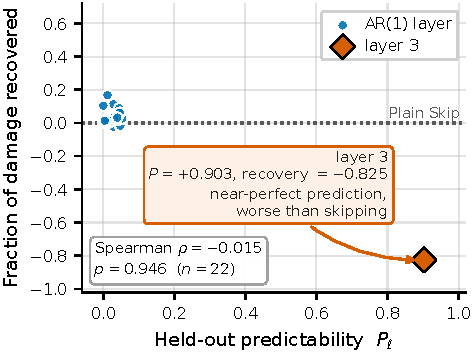
\includegraphics[width=0.78\linewidth]{figures/fig1b_recovery_vs_P.pdf}
\caption{\textbf{Predictability does not imply recoverability.} For each eligible layer of
Qwen2.5-0.5B: held-out explained update energy $P_\ell$ (\cref{eq:pscore}) against the
fraction of that layer's single-layer plain-skip NLL damage the scalar predictor repairs.
The two are unrelated (Spearman $-0.015$, $p=0.946$, $n=22$). Layer~3, the \emph{most} predictable layer in the network ($P_\ell=0.90$), is the worst to
predict: substituting that near-perfect forecast is markedly worse than dropping the update
outright (recovery $-0.825$). Hardware and protocol: \Cref{sec:app-protocol}. Depth profile:
\Cref{fig:momentum-profile}.}
\label{fig:momentum}
\end{figure}


\subsection{Predictability across depth}
\begin{figure}[t]
\centering
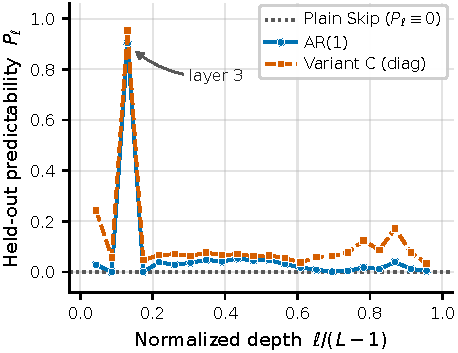
\includegraphics[width=0.62\linewidth]{figures/fig1a_predictability.pdf}
\caption{\textbf{Predictability across depth.} Held-out explained update energy $P_\ell$
against normalized depth in Qwen2.5-0.5B, for the scalar predictor (\cref{eq:ar1}) and
for \mname (\cref{eq:diag}); plain skipping is the $P_\ell \equiv 0$ baseline. The
per-channel predictor explains more of the update at nearly every depth, and layer~3
sits far above the rest at $P_\ell=0.90$, the layer that
\Cref{fig:momentum} shows is the worst of all to predict. Hardware and protocol: \Cref{sec:app-protocol}.}
\label{fig:momentum-profile}
\end{figure}


The depth profile behind \Cref{fig:momentum} is shown in \Cref{fig:momentum-profile}.

\subsection{Light-budget downstream results}
\begin{table}[t]
\centering
\small
\setlength{\tabcolsep}{3pt}
\caption{\textbf{Light budgets: no accuracy difference is significant.} The 0.5B and 1.5B rows,
at $k \le 4$ under damage-based selection. \mname wins the NLL column throughout; no accuracy
difference reaches significance at any budget or scale here (largest $|z|=1.18$), consistent
with the necessity rule of \Cref{sec:experiments}: these cells do not carry enough damage for
repair to pay off downstream. Counts in parentheses are net correct answers against Plain Skip,
out of 300 on 0.5B and 900 on 1.5B. Hardware and protocol: \Cref{sec:app-protocol}.}
\label{tab:light}
\begin{tabular}{llcccccc}
\toprule
Method & $k/L$ & NLL $\downarrow$ & HellaSwag & PIQA & ARC-E & Avg. & Gap rec. \\
\midrule
\multicolumn{8}{c}{\textit{\cellcolor[HTML]{EFEFEF}Qwen2.5-0.5B ($L=24$)}} \\
\midrule
Dense                  & 0/24 & 2.76 & 48.0 & 68.0 & 60.0 & 58.7 & \\
\graymidrule
Plain Skip             & 2/24 & 2.98 & \textbf{44.0} & \textbf{66.0} & \textbf{48.0} & \textbf{52.7} &  \\
Copy Update            & 2/24 & 3.41 & 39.0 & 64.0 & 47.0 & 50.0 & -44.4\%\ (-8) \\
Scalar AR(1)           & 2/24 & 2.97 & 43.0 & 64.0 & \textbf{48.0} & 51.7 & -16.7\%\ (-3) \\
\textbf{\mname (Ours)} & 2/24 & \textbf{2.97} & 41.0 & 64.0 & \textbf{48.0} & 51.0 & -27.8\%\ (-5) \\
\graymidrule
Plain Skip             & 4/24 & 3.42 & \textbf{42.0} & \textbf{68.0} & \textbf{47.0} & \textbf{52.3} &  \\
Copy Update            & 4/24 & 5.08 & 31.0 & 54.0 & 42.0 & 42.3 & -157.9\%\ (-30) \\
Scalar AR(1)           & 4/24 & 3.41 & 40.0 & \textbf{68.0} & 46.0 & 51.3 & -15.8\%\ (-3) \\
\textbf{\mname (Ours)} & 4/24 & \textbf{3.39} & 40.0 & 66.0 & \textbf{47.0} & 51.0 & -21.1\%\ (-4) \\
\midrule
\multicolumn{8}{c}{\textit{\cellcolor[HTML]{EFEFEF}Qwen2.5-1.5B ($L=28$)}} \\
\midrule
Dense                  & 0/28 & 2.33 & 67.3 & 73.7 & 73.0 & 71.3 & \\
\graymidrule
Plain Skip             & 2/28 & 2.47 & 61.7 & 73.3 & 70.0 & 68.3 &  \\
Copy Update            & 2/28 & 2.83 & 58.0 & \textbf{76.0} & 57.3 & 63.8 & -151.9\%\ (-41) \\
Scalar AR(1)           & 2/28 & 2.46 & \textbf{62.7} & 73.3 & 70.0 & 68.7 & +11.1\%\ (+3) \\
\textbf{\mname (Ours)} & 2/28 & \textbf{2.46} & \textbf{62.7} & 73.3 & \textbf{70.7} & \textbf{68.9} & +18.5\%\ (+5) \\
\graymidrule
Plain Skip             & 4/28 & 2.75 & \textbf{51.0} & \textbf{72.7} & \textbf{68.0} & \textbf{63.9} &  \\
Copy Update            & 4/28 & 4.46 & 34.3 & 60.7 & 37.3 & 44.1 & -265.7\%\ (-178) \\
Scalar AR(1)           & 4/28 & 2.71 & \textbf{51.0} & 72.3 & 67.3 & 63.6 & -4.5\%\ (-3) \\
\textbf{\mname (Ours)} & 4/28 & \textbf{2.71} & \textbf{51.0} & 71.7 & 67.7 & 63.4 & -6.0\%\ (-4) \\
\bottomrule
\end{tabular}
\end{table}


\subsection{Full downstream results}
\label{sec:app-downstream}



\subsection{Accuracy deltas, sampling noise, and ratio inflation}
\label{sec:app-noise}

Recovered-gap \emph{fractions} on accuracy divide by a Dense-minus-Plain-Skip denominator
only tens of graded answers wide, and are correspondingly unstable. We therefore tested
every \mname-versus-Plain-Skip accuracy comparison against the standard error of a
difference of two proportions, and report absolute counts in the body. Of the 63
comparisons, 59 are not significant at the two-sided $95\%$ level. A $1$-SE band is
not a significance test: a delta at $1.0$--$1.2$ SE has $p \approx 0.25$ and establishes
nothing.

Only 4 comparisons are significant, and both survive Bonferroni correction over the
family of 63 tests actually performed ($\alpha/m = 0.00079$, $|z| \ge
3.35$): recovery-maximising selection on Qwen2.5-1.5B at $k=2$
($+132$ answers, $z=6.45$) and $k=4$ ($+90$, $z=4.37$). Both are
earned on models plain skipping has already destroyed. Correction matters here rather
than being ceremonial: an uncorrected $95\%$ threshold over 63 tests would expect
about 3.15 false positives by chance, so the uncorrected borderline case
(0.5B, recovery-top, $k=2$, $z=1.95$) cannot be claimed.

\paragraph{A third source of uncertainty: the evaluation is not deterministic.} Binomial
sampling error is not the only noise in these numbers. Re-scoring an \emph{identical}
configuration under a different task batch shape changes the score. Language-modelling NLL is
identical up to fp64 accumulator roundoff (maximum $|\Delta\mathrm{NLL}| =
4.44e-16$, one ulp), but multiple-choice items whose top two options are nearly tied can
flip, because BF16 matmul reduction order depends on batch shape and perturbs the logits at
the last bit. Duplicating one configuration (Qwen2.5-1.5B, damage-selected $k=2$,
seed 42, same layers, evaluated once at 32 rows per batch and once at 8) moves up
to 4 answers of 900, with nothing else changed. That is the same magnitude as
\emph{every} accuracy difference we report at the deployable operating point. Those
differences are therefore below the reproducibility floor of the evaluation itself, not merely
inside sampling error. We do not regard this as a weakness of the analysis: it locates the
floor, and our refusal to claim either an improvement or a regression there sits exactly on
it.

The Bonferroni survivors are unaffected, and we state the ratio rather than assert immunity.
Four of 63 comparisons survive correction: Qwen2.5-7B under damage-based selection at
$k=8$ (89 answers, $z=4.31$; and 74 for the cross-token extension,
$z=3.57$), and Qwen2.5-1.5B under damage-seeking selection at $k=2$ and $k=4$
(132 and 90 answers, $z=6.45$ and $4.37$). Measured against the replicated BF16 floor (a maximum of 6
answers of 900), the four survivors are 22.0, 15.0, 14.8 and 12.3 times that floor. No
reordering of the evaluation batch produces effects of that size.

\paragraph{The axis is damage, not selection rule.} Across all 28 skipping runs in this
paper, the recovery \mname achieves correlates with the damage plain skipping does: Spearman
$\rho = 0.820$ ($p = 9.0e-08$) between plain-skip NLL damage and \mname's NLL
gain, and $\rho = 0.468$ ($p = 0.012$) on the accuracy axis. \emph{We report this
as descriptive ordering, not as a fitted law.} The 28 runs are not independent: budgets
are nested, models are shared, and gain and damage share terms by construction, so the
correlation coefficient should not be read as an effect size. The robust evidence is the
enumeration rather than the statistic: the five largest gains all occur in high-damage runs,
and every low-damage run is null. The aphorism summarizes that ordering; it does not
extrapolate beyond it.

We apply the significance test symmetrically. A delta inside the noise band is discounted
whichever way it points, so we neither credit \mname with the $+18.5\%$ that five answers
produce at
$k=2$ on 1.5B, nor charge it with the $-6\%$ that four answers produce at $k=4$.

\subsection{The two selection rules are the dissociation}
\label{sec:app-tworules}

So the two selection rules \emph{are} the dissociation. The rule that maximises measured
recovery earns \mname's largest likelihood recovery anywhere (70.0\% at $k=2$ on
1.5B, at an absolute loss of 3.43 against a dense 2.33) and its only
significant accuracy gains, on models whose absolute quality is unacceptable. The rule
that keeps quality acceptable earns a real likelihood recovery (23.3\% at $k=4$ on
7B) and no significant accuracy effect at all. Recovery and functional repair agree only once the
model is already ruined enough for there to be something obvious to repair. The
depth-wise anti-correlation underlying this is quantified in \Cref{sec:app-anticorr}.

\subsection{Why the per-channel predictor wins is not settled}
At layer 3 the fitted scalar is $+1.10$ while the median channel coefficient is
$-0.20$ and 76\% of channels are negative, so the scalar moves three quarters of
the channels the wrong way. That cannot be the whole story, since \mname also beats the
scalar at layers whose channels agree in sign.

\subsection{The cross-token extension: depth is not the only cheap signal}
\label{sec:app-crosstoken}

\Cref{eq:diag} predicts a skipped block's update from the previous layer's update at the
\emph{same} token position. Nothing forces that choice. Giving each channel a second
coefficient on the preceding layer's update at the preceding \emph{token},
\begin{equation}
\widehat{\dd}_\ell(t) = \aal_\ell \odot \dd_{\ell-1}(t) + \bb_\ell \odot \dd_{\ell-1}(t-1),
\label{eq:crosstoken}
\end{equation}
costs 1792 scalars per skipped block on Qwen2.5-0.5B. This is \emph{twice the
coefficient storage of \mname proper, and still $O(Td)$ compute}: the shifted tensor is
already resident in the residual stream, so no extra matmul is introduced. We keep the two
separate throughout, and every claim about \mname elsewhere in this paper refers to the
$d$-parameter predictor of \cref{eq:diag}. Setting $\bb_\ell = \bm{0}$ reduces
\cref{eq:crosstoken} to \cref{eq:diag} exactly, which we verify numerically (0.0
absolute NLL difference).

On a single-layer scan over the 22 eligible layers of Qwen2.5-0.5B, cross-token
prediction lowers mean held-out NLL from 3.40 to 3.08 against a dense
2.76, and beats the depth-only predictor at 19 of the 22 layers, raising
median single-layer recovery by 1.8$\times$.

The most informative case is the one no ridge could fix. Layer 2 is where the per-channel
predictor is at its most destructive, and regularisation does not rescue it: across four
orders of magnitude of ridge strength its recovery never rises above $-2.42$
(\Cref{sec:app-ridge}), and it sits at $-3.31$ at the fitted value. Admitting the
previous token's update turns that same layer from $-3.31$ to $+0.19$. The
failure was missing information, not mis-regularisation.

\paragraph{Composition: cross-token matches the depth-only predictor, and the reason is
instructive.} At the deployable, damage-selected layer sets, cross-token prediction does not
improve on \cref{eq:diag} in any way that matters. On Qwen2.5-0.5B it recovers 4.8\%
of the plain-skip NLL damage at $k=4$ against 4.6\% for the depth-only predictor, and
18.3\% against 18.0\% at $k=6$; on Qwen2.5-1.5B, 8.9\% against 8.2\%
at $k=2$ and 10.8\% against 10.3\% at $k=4$. Downstream accuracy is at noise
level in both directions, so the dissociation this paper reports extends to the cross-token
predictor as well.

The reason is measurable rather than mysterious, and it is the same selection story told
once more. Cross-token information rescues precisely the layers that damage-aware selection
has already discarded: its three largest gains over \cref{eq:diag} are at layers 2,
21 and 1, while the deployable sets are $\{8,10,13,18\}$ and
$\{10,12,14,16\}$. The two are disjoint. A selection rule that avoids catastrophic layers
gets, for free, the layers on which the cheaper predictor was already adequate, so the extra
information has nothing left to repair.

What cross-token buys at the deployable sets is therefore not recovery but
\emph{robustness}: its worst layer anywhere in the scan recovers $-0.027$, against
$-3.314$ for the depth-only predictor. It removes the failure mode rather than
improving the typical case.

\paragraph{A pre-registered test of the damage axis.} Cross-token selection provides a test of
the damage ordering rather than another illustration of it. Before running it we predicted
that selecting layers by cross-token recovery would produce high-damage sets, and that the
damage axis therefore expected a large cross-token gain there. On likelihood the prediction
holds: these are the most damaged sets in the paper (plain-skip NLL 6.59 at $k=2$ and
9.58 at $k=4$, against a dense 2.76), and the cross-token extension recovers
66.8\% and 63.7\% of that damage, its largest recoveries anywhere and roughly ten
points above the depth-only predictor's 56.3\% and 54.7\%. Accuracy moves in the predicted direction as well, by
16 to 23 correct answers of 300, but at this sample size it is
under-powered and we claim no significance for it. The prediction is confirmed on the
likelihood axis and untested on the accuracy axis, and we say so rather than reading the
accuracy counts as support.

We report all of this as preliminary at one scale for the single-layer scan, and we make no
claim that cross-token prediction improves \mname at a deployable operating point. Its value
in this paper is the mechanism: it identifies what the depth-only predictors were missing.

\subsection{The dissociation view}
\begin{figure*}[t]
\centering
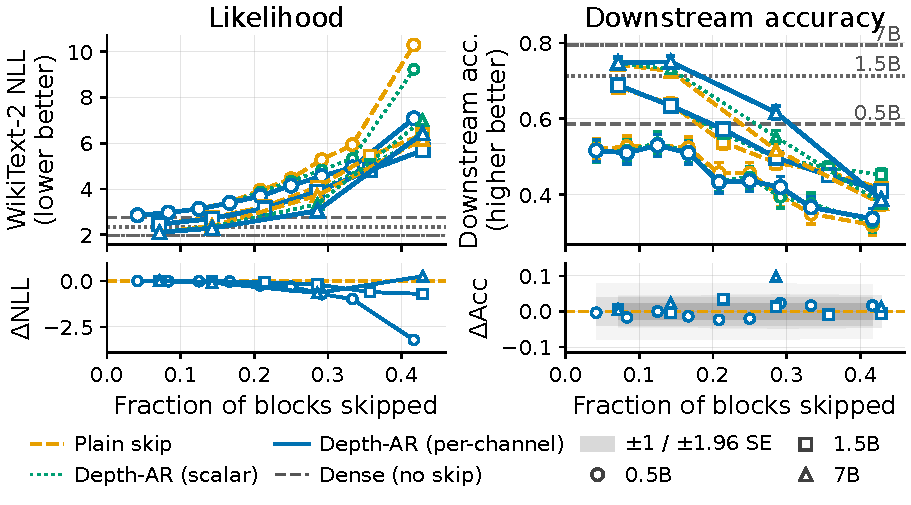
\includegraphics[width=0.62\textwidth]{figures/fig2_dissociation.pdf}
\caption{\textbf{Significant gains appear only where skipping does severe damage.} Quality against
the fraction of blocks skipped, for Qwen2.5-0.5B (circles), 1.5B (squares) and 7B (triangles),
with layers chosen by measured residual damage and every predictor skipping the identical
blocks. Lower panels plot the difference against plain skipping directly, so a point below zero
on the left is an improvement in likelihood and a point above zero on the right is an
improvement in accuracy. Shaded bands are $\pm 1$ and $\pm 1.96$ binomial standard errors.
Where skipping barely hurts, at the left of each panel, \mname and plain skipping are
indistinguishable in behaviour, and the differences there are smaller than the evaluation's own
measured reproducibility floor. Where skipping does severe damage the gap opens: at 28.6\% of
blocks skipped on 7B, \mname answers 89 more questions correctly out of 900 than plain skipping
($z=4.31$, surviving Bonferroni correction across all 63 comparisons) while recovering 38.1\%
of its language-modelling damage. Both breakdowns are drawn rather than hidden: at 42.9\%
skipped on 7B the depth-only predictor falls \emph{below} plain skipping on likelihood, where
the cross-token extension does not. Hardware and protocol: \Cref{sec:app-protocol}.}
\label{fig:dissociation}
\end{figure*}


The same data as \Cref{fig:gains-pair}, drawn as paired likelihood and accuracy panels.

\subsection{The quality-compression frontier}
\label{sec:app-pareto}

\Cref{fig:dissociation} plots quality against the fraction of blocks skipped. The underlying
cells, at damage-based selection, are below; recovery-maximising selection is excluded, since
the models it produces are not ones anyone would deploy. \mname's advantage over plain
skipping widens as compression deepens on Qwen2.5-0.5B and Qwen2.5-1.5B.

It does not widen forever. On Qwen2.5-7B at 42.9\% of blocks skipped, the depth-only
predictor \emph{breaks down}: it recovers $-6.0$\% of the plain-skip damage, which is to
say it is worse than simply dropping the updates (NLL 6.43 against plain skipping's
6.18). We report this rather than truncating the sweep at the last budget that flatters
the method. At that same point the cross-token extension remains above plain skipping
(7.1\% recovery, NLL 5.88), and this is the closing half of the selection story
told earlier. At mild budgets, damage-aware selection avoids the early layers on which
cross-token information helps, so the extension has nothing to add. At 42.9\% skipped
the budget \emph{forces} those layers into the set (it contains layers 1 and 3), and the extra
information finally expresses itself. Cross-token prediction matters exactly where prediction
is hardest, which is also exactly where the depth-only predictor fails.

\begin{table}[h]
\centering
\small
\caption{\textbf{Frontier cells at damage-based selection.} NLL on WikiText-2 test; recovered
is the fraction of plain-skip damage repaired. A negative value is worse than dropping the
updates. \mname is the depth-only predictor of \cref{eq:diag}; CT is the cross-token extension
of \Cref{sec:app-crosstoken}, evaluated only where it was run.}
\label{tab:pareto}
\begin{tabular}{llccccc}
\toprule
Model & $k$ & skipped & Plain NLL $\downarrow$ & \mname NLL $\downarrow$ & \mname rec. $\uparrow$ & CT rec. $\uparrow$ \\
\midrule
0.5B & 6 & 25.0\% & 4.45 & 4.15 & 18.0\% & {--} \\
0.5B & 8 & 33.3\% & 5.93 & 4.94 & 31.3\% & {--} \\
0.5B & 10 & 41.7\% & 10.29 & 7.09 & 42.6\% & {--} \\
1.5B & 6 & 21.4\% & 3.24 & 3.16 & 8.6\% & {--} \\
1.5B & 8 & 28.6\% & 4.08 & 3.89 & 11.1\% & 11.6\% \\
1.5B & 10 & 35.7\% & 5.43 & 4.83 & 19.6\% & 19.8\% \\
1.5B & 12 & 42.9\% & 6.39 & 5.69 & 17.3\% & 17.4\% \\
7B & 8 & 28.6\% & 3.71 & 3.05 & 38.1\% & 38.1\% \\
7B & 12 & 42.9\% & 6.18 & 6.43 & -6.0\% & 7.1\% \\
\bottomrule
\end{tabular}
\end{table}

\subsection{External validity: the Qwen3 family}
\begin{table}[t]
\centering
\small
\caption{\textbf{A second model family.} Qwen3 at the deployable budget ($k=4$, damage-based
selection), same protocol as Qwen2.5-1.5B/7B. Recovery is non-monotone in model size: the
Qwen2.5 scale trend is family-specific, not universal. Qwen3-1.7B is the diagnosed exception,
where four layers that each repair to better than dense individually fail to compose
(\Cref{sec:app-qwen3}).}
\label{tab:qwen3main}
\begin{tabular}{lccc}
\toprule
Model & Damage (nats) & \mname rec. & CT rec. \\
\midrule
Qwen3-1.7B & 0.61 & -1.9\% & -2.7\% \\
Qwen3-4B & 0.10 & +4.7\% & +6.2\% \\
Qwen3-8B & 0.16 & +12.7\% & +13.2\% \\
\bottomrule
\end{tabular}
\end{table}


\label{sec:app-qwen3}

Everything above is measured on the Qwen2.5 family. To test whether the scale trend and the
damage ordering are properties of Transformers or of that family, we ran the deployable
configuration ($k=4$, damage-based selection) on Qwen3 at 0.6B, 1.7B, 4B and 8B, under the
identical protocol used for Qwen2.5-1.5B and 7B: BF16 on a single NVIDIA RTX 3090, 32
calibration sequences of length 1024 from WikiText-103, NLL on the WikiText-2 test split.

\textbf{The scale trend does not replicate.} Recovery is non-monotone in model size across the
Qwen3 ladder: $+20.5\%$ at 0.6B, $-1.9\%$ at 1.7B, $+4.7\%$ at 4B and $+12.7\%$ at 8B. The
growth with scale we report on Qwen2.5 at $k=4$ is therefore a property of that family, not a
general property of Transformer depth, and we scope the claim accordingly rather than confining
our evidence to the family that shows it. The three low-damage cells are consistent with the
damage ordering; 1.7B is the exception, and it is the diagnosed one.

\textbf{The cross-token advantage does replicate.} On every Qwen3 model where either predictor
works at all, the cross-token extension beats the per-channel predictor: $+21.2\%$ against
$+20.5\%$ at 0.6B, $+6.2\%$ against $+4.7\%$ at 4B, and $+13.2\%$ against $+12.7\%$ at 8B. At
1.7B, the compounding-failure cell, both predictors fail and cross-token fails slightly worse
($-2.7\%$ against $-1.9\%$). The extension's advantage therefore transfers to a second family,
while the failure mode transfers with it.

\textbf{The damage ordering does not transfer cleanly either, and the exception is the sharpest
one available.} Qwen3-1.7B is the \emph{most} damaged of the three cells (plain skipping costs
0.61 nats) and it is the one where \mname recovers nothing at all. On our Qwen2.5 runs, damage
of that size is where recovery is largest. Qwen3-4B is the least damaged (0.10 nats) and shows
the small gain the ordering would predict, and 0.6B is consistent as well, so the failure is
specific rather than total.

The exception has a measured mechanism. Each of the four layers selected at 1.7B repairs, on
its own, to \emph{better than dense}: their post-repair NLL deltas are $-0.063$, $-0.044$,
$-0.033$ and $-0.026$. Composed, the same four layers cost 0.61 nats that repair does not
recover. Single-layer gains failed to compose. This is precisely the compounding failure our
non-adjacency constraint (a gap of at least two surviving blocks between skipped ones) was
designed to prevent, and it is observed here in spite of it. That partially rescues the damage
ordering: what fails at 1.7B is composition, not the relation between damage and repair.
Whether it rescues it enough is not something three cells can settle, and we do not claim it
does. The correlation of \Cref{sec:app-noise} remains what we said it was: a description of the
runs we performed, not a law.

We also note an interaction we cannot resolve with the evidence we have. Within Qwen2.5 at the
deployable budget, plain-skip damage \emph{falls} with model size while recovery \emph{rises}
with it, so size and damage push in opposite directions there and our runs cannot separate their
contributions. The Qwen3 ladder, where damage does not decrease monotonically with size, does
not settle it either. Disentangling model size, skipping damage and model family is future work,
and we make no claim about their interplay.

\paragraph{A note on ratios with vanishing denominators.} Recovery fractions are undefined when
plain skipping does no damage. At 1.7B, several individual layers are \emph{better} skipped
than kept (layer 12's removal improves NLL by 0.017), and a recovery fraction computed against
that near-zero, wrong-signed denominator reads $-1.61$ while the repaired model is in fact
0.044 better than dense. We therefore report post-repair NLL deltas, not recovery fractions,
for any cell whose damage is non-positive. A ratio is only as meaningful as its denominator,
and this is the second time in this work that a small denominator produced a large and empty
number (\Cref{sec:app-noise}).

\begin{table}[h]
\centering
\small
\caption{\textbf{Qwen3, deployable configuration ($k=4$, damage-based selection).} Damage is the
NLL cost of plain skipping. CT is the cross-token extension. Recovery is non-monotone in scale,
and is absent at 1.7B despite that cell being the most damaged.}
\label{tab:qwen3}
\begin{tabular}{lccccc}
\toprule
Model & Dense NLL & Plain Skip NLL & Damage (nats) & \mname rec. & CT rec. \\
\midrule
Qwen3-0.6B & 3.17 & 3.61 & 0.44 & +20.5\% & +21.2\% \\
Qwen3-1.7B & 2.91 & 3.53 & 0.61 & -1.9\% & -2.7\% \\
Qwen3-4B & 2.71 & 2.81 & 0.10 & +4.7\% & +6.2\% \\
Qwen3-8B & 2.38 & 2.54 & 0.16 & +12.7\% & +13.2\% \\
\end{tabular}
\end{table}

\subsection{Layer selection}

\label{sec:app-selection}

The three selection rules of \Cref{tab:selection} are: (i) \emph{predictability},
ranking layers by held-out $P_\ell$ (\cref{eq:pscore}), which requires only a
forward pass of the dense model and no skipping; (ii) \emph{lowest single-layer
damage}, ranking by the NLL increase caused by skipping each layer individually on
the development set; and (iii) \emph{measured recovery}, ranking by the fraction of
that damage the predictor repairs. Rules (ii) and (iii) require one forward pass
per candidate layer and are correspondingly more expensive than (i); only (i) is
free. That (i) is also the rule that fails is the practical sting of
\Cref{sec:experiments}. All rules enforce the same non-adjacency constraint, and
all predictors are compared at the identical layer set a rule produces.

\clearpage
\section{Archival detail}
\label{sec:app-archival}

\emph{This appendix is supporting material and may be removed without affecting any claim in the
paper. No statement in the body or in \Cref{sec:app-experiments} depends on it; we verified this
mechanically.}
\subsection{Two taps buy nothing}
\label{sec:app-ar2}

We also evaluated a two-tap variant, $\widehat{\dd}_\ell = \alpha_\ell \dd_{\ell-1}
+ \beta_\ell \dd_{\ell-2}$, fitting $(\alpha_\ell, \beta_\ell)$ through a
$2\times2$ ridge system. Averaged over the eligible layers of Qwen2.5-0.5B it
improves single-layer recovery over the one-tap scalar by $+0.0009$, that
is, not at all. The information a second tap adds is negligible next to the
information a second \emph{channel} adds, which is the point of \cref{eq:diag}: the
useful axis of capacity here is across the hidden width, not back along depth. We
therefore report the one-tap predictor throughout and do not pursue longer windows.

\subsection{Implementation and correctness checks}
\label{sec:app-correctness}

\mname is implemented as a wrapper around the decoder stack that intercepts the
residual update of each block. Before running any experiment we verified the
wrapper with six checks, all of which pass on Qwen2.5-0.5B (24 blocks, 22
eligible). The dense wrapper reproduces the unmodified model's logits
\textbf{bit-exactly} (maximum absolute logit difference $0.0$), as do the
$\aal_\ell = \bm{0}$ reduction to Plain Skip (checked at layers 5, 9 and
13) and a hand-written single-layer skip (layer 9). Residual updates are
captured at the block boundary of \cref{eq:residual} to a maximum absolute error of
$3.8 \times 10^{-6}$ against a hidden-state scale of $1.7 \times 10^{3}$.
Scrambling the padded token slots moves neither the fitted accumulators nor the
held-out NLL ($0.0$ change, 192 real tokens counted), confirming that
padding is excluded from \cref{eq:fit}. The selected layer set is non-adjacent by
construction (minimum gap 2, first and last blocks excluded).

